\documentclass[conference]{IEEEtran}
\usepackage{changepage}
\usepackage{multicol}
\usepackage{wrapfig}
\usepackage{amsmath,amssymb,amsfonts}
\usepackage{algorithmic}
\usepackage{graphicx}
\usepackage{textcomp}
\usepackage{xcolor}
\usepackage{array}
\usepackage{ragged2e}
\usepackage{float} % Appending the [H] option forces the placement of a figure in the place it's in the code
\usepackage{pdfpages}

\begin{document}
\title{Lab 4 Report --- Completed CR16 Processor\\
\Large{Computer Design Laboratory ECE 3710}\\
\Large{Fall 2021}\\
\Large{The University of Utah}}

\author{\IEEEauthorblockN{Jacob Peterson}
\IEEEauthorblockA{\textit{Computer Engineering 2022}\\
\textit{University of Utah}\\
Salt Lake City, UT}
\and
\IEEEauthorblockN{Brady Hartog}
\IEEEauthorblockA{\textit{Computer Engineering 2022}\\
\textit{University of Utah}\\
Salt Lake City, UT}
\and
\IEEEauthorblockN{Isabella Gilman}
\IEEEauthorblockA{\textit{Computer Engineering 2023}\\
\textit{University of Utah}\\
Salt Lake City, UT}
\and
\IEEEauthorblockN{Nate Hansen}
\IEEEauthorblockA{\textit{Computer Engineering 2023}\\
\textit{University of Utah}\\
Salt Lake City, UT}
}

\maketitle
\begin{abstract}
\textbf{This report focuses on the final design steps of the 16-bit compact RISC (CR16) processor. The module we designed integrates the datapath, register file, and Block RAM to a Finite State Machine that controls the loading and execution of program instructions. We can decode and execute instructions in a single state, and then transition based on instruction type. To manage the exceptional control flow, we implemented a program counter that has various functions in addition to incrementing after each execute state. We made a few adjustments to our implementation of the datapath, detailed hereafter. We adopted a custom ISA that is similar to the one provided for a compact RISC design to the University of Utah's ECE 3710 class. We will address briefly about how we plan to assemble instructions from the ISA. We intend to use this project as the driver for a Fully-Synchronized Synthesizer interface (FSS).}
\end{abstract}

\section{Introduction}
Throughout the design process for the CR16 processor, we have come to understand and adapt its functionality towards our specific application in the FSS. As such, we have modified various aspects of our previous incremental design multiple times.We will report on these changes and decisions, and hopefully provide some insight into our design process. We defined a few capabilities that we need our CR16 CPU to have. 

\begin{enumerate}
    \item The CR16 must be able to interface with the GPIO registers and the I2C controller on the FPGA.
    \item The Processor must be fast enough to interface with the audio CODEC over I2C, poll for the state of the inputs on the FSS over GPIO, and update the state of some LEDs on the FSS in a reasonable timeframe.
    \item The ISA we construct for the CR16 should be something that makes sense to every group member. Instructions should be intuitive, and the FSM implementation of each instruction type should operate efficiently.
    \item The conventions and rules of the ISA and the hardware should be well-defined for ease of code development.
\end{enumerate}

Using this short set of goals, we set out to integrate BRAM, the datapath, and the program counter with an FSM that would control the flow of a preloaded software program.

\section{Changes to the Datapath}

\begin{figure}[ht]
    \centering
    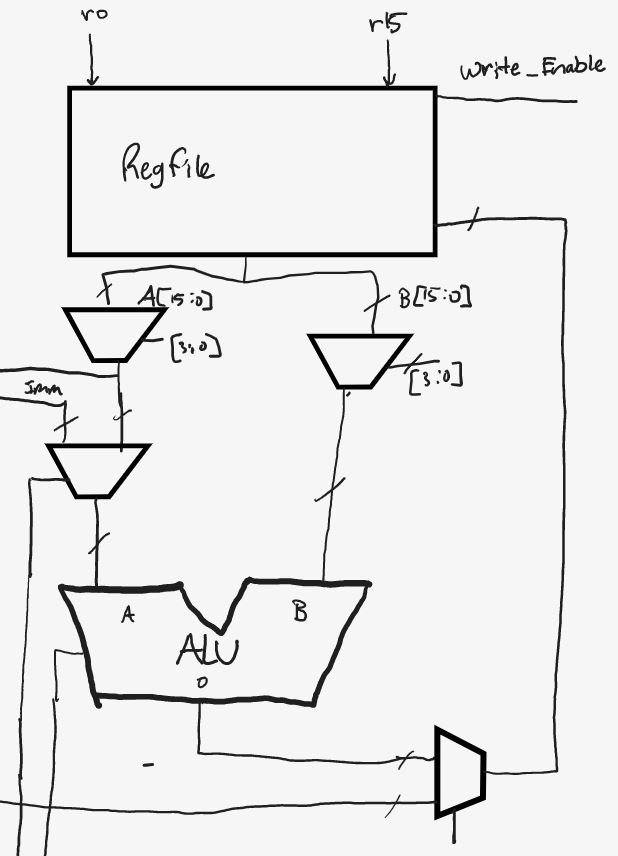
\includegraphics[scale=0.55]{resources/figures/datapath.jpg}
    \caption{The most recent block diagram of our cr16 datapath. Some labels removed for simplicity.}
    \label{fig:datapath}
\end{figure}

\begin{figure*}[t]
    \centering
    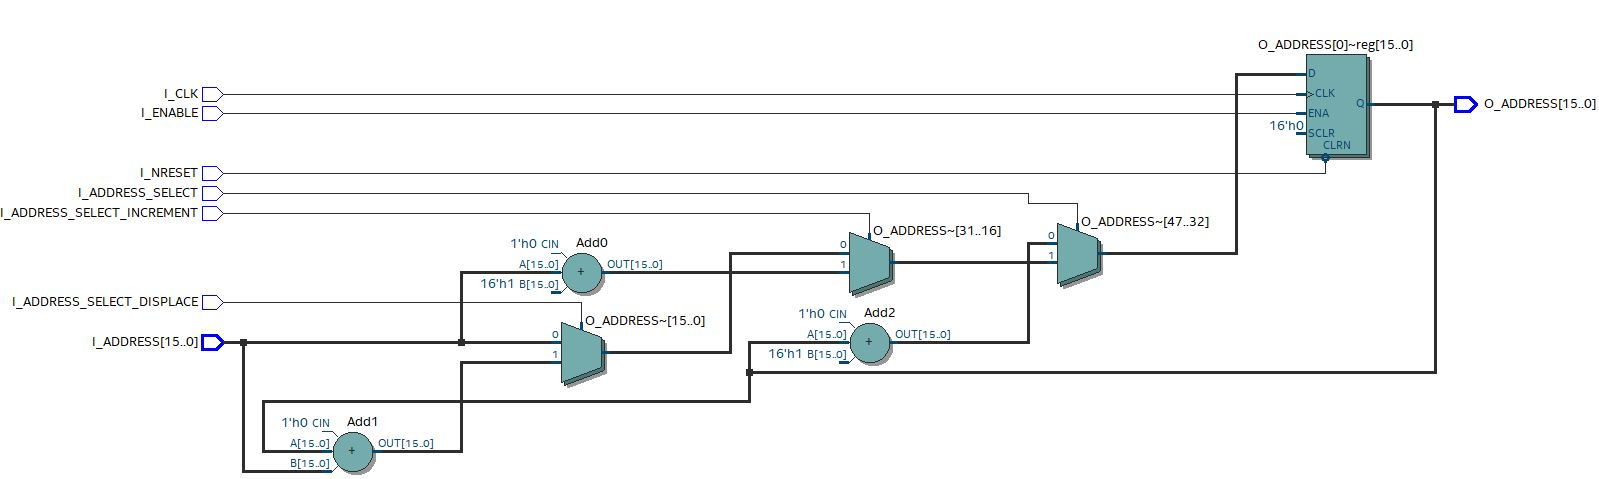
\includegraphics[scale=0.5]{resources/figures/program_counter.jpg}
    \caption{Block diagram for the program counter module}
    \label{fig:program_counter}
\end{figure*}

We made various changes to our previous implementation of the datapath in order for it to function properly in concert with the FSM. The block diagram of our most recent design for the datapath is contained in Fig. \ref{fig:datapath}. The modified modules were tested with their respective testbenches, which in some cases needed to be modified as well. The changes were as follows:
\begin{enumerate}
    \item \textit{Added a multiplexer with the ALU output data line to directly load data into the regfile and bypass the ALU.} This was done to facilitate LOAD/MOV type instructions. 
    \item \textit{Consolidate ALU Opcodes.} The way we had initially built our ALU to set flags was flawed for various reasons. We established a new method to do that more efficiently. We eliminated some ALU opcodes that were repetitive, and only the opcodes corresponding to SUB, ADDC, and ADD will set flags. Since writeback to the regfile is a concern of the FSM, the CMP and CMPI instructions will use the SUB opcode on the ALU to trigger the appropriate flags. The three instructions mentioned above will modify all the applicable flags. However, for the sake of consistency in the code, we should only use CMP/CMPI by convention for setting Jcond/Bcond condition codes.
    \item \textit{Moved multiplexing immediate operands to input A.} By convention, we have assigned Rdest to correspond to ALU input B and Rsrc to correspond to ALU input A. It is a concern of the FSM to select an immediate operand from the instruction or a data value from the regfile to place on ALU input A.
    \item \textit{Add a direct output from the regfile at read port A.} This direct output allows the STORE instruction to access the regfile directly and select the register data to store in memory through Rsrc.
\end{enumerate}

These changes have significantly cleaned up our code and allowed us to set some programming conventions. We hope this will make the programming process as smooth as possible. 

\section{Design Decisions for the ISA}
In order to proceed with the design of the FSM, we need to establish an exact ISA. This will allow us to write logic to decode instructions properly. We made a few modifications to the ISA provided to us so we could implement some desired behavior.
\begin{enumerate}
    \item \textit{LOADX/STOREX:} These instructions are external LOAD and STORE instructions which will be capable of storing data directly into an external register. This was implemented for two reasons. We want LOAD and STORE to have access to the whole address space of instantiated BRAM, and we want to be able to communicate in a modular way with GPIO resgisters that are sending information to the audio CODEC over I2C.
    \item \textit{CALL/CALLD/RET instead of JAL/JUC:} Our software will potentially be quite long, and those of us who will be writing it want to use the stack to manage subroutine calls within subroutine calls. It seems to make more logical sense to encapsulate the management of the stack within an instruction. The CALL and CALLD (CALL with displacement) instructions will manage the return address implicitly, and RET will be an unconditional jump to the previously calculated return address. This way, we don't need a dedicated register for the return address.
    \item \textit{PUSH/POP:} These instructions will encapsulate the behavior of modifying the stack pointer and loading/storing data in the stack. Although we haven't implemented them yet, we believe this instructions could be useful.
\end{enumerate}
It is important to note that if the state machine in the FSM becomes too complicated due to the behavior of any of these instructions, we will fall back on the simpler behavior of the provided ISA. The software is likely to be the most burdensome aspect of our project, so we want to develop it intuitively and cleanly. The full ISA is located in Appendix Table 1.

\section{The Program Counter}
The program counter module is designed to increment the program counter naturally after the execution of each instruction. This module is depicted in Fig. \ref{fig:program_counter}. Multiple complications to the advancement of the program counter arise from the non-linear control flow of jumps, branches, and method calls. In order to handle this, the program counter module has some additional logic. Our program counter supports both direct modification of the program counter and 2's complement signed displacement of the program counter. The input I\_ADDRESS\_SELECT multiplexes between the natural incrementing of the PC and a user-defined input as seen on I\_ADDRESS. The I\_ADDRESS\_SELECT\_DISPLACE multiplexes between the natural incrementing of the PC and adding a 2's compliment displacement seen on I\_ADDRESS. The input I\_SELECT\_INCREMENT multiplexes between propagating I\_ADDRESS to O\_ADDRESS and propagating I\_ADDRESS + 1 to O\_ADDRESS. We implemented the increment selector as a way to return to the correct address after a method call. This may be done in other ways, but this seemed to simplify the FSM code. This PC setup should allow for all types of conditional control flow available in our ISA.

\section{Decoding and Executing Instructions}
With all of the opcodes and instruction behavior established, we are prepared to design and implement an FSM that will fetch, decode, and execute instructions that are pre-loaded to the BRAM module through a memory initialization file. 

\begin{figure}[ht]
    \centering
    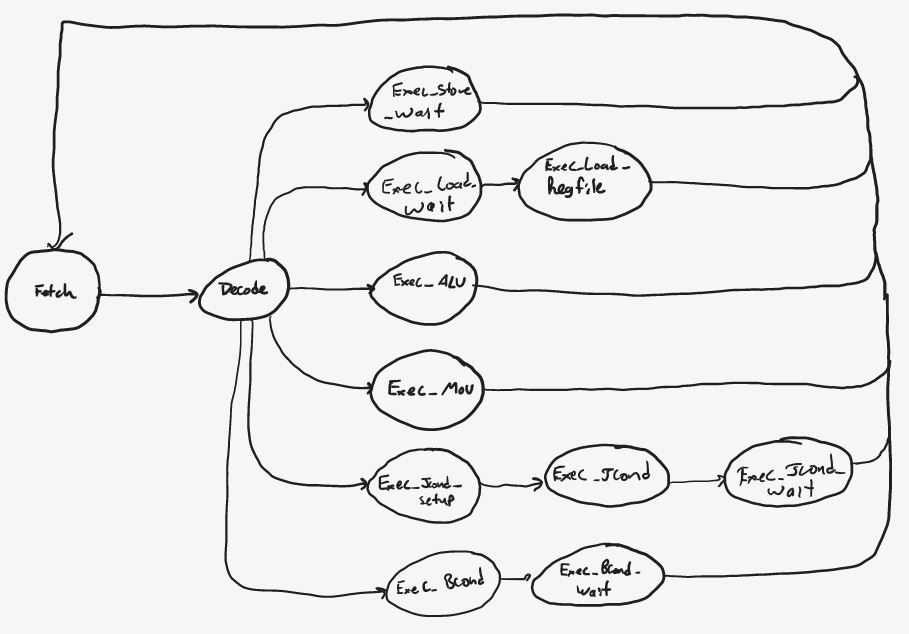
\includegraphics[scale=0.45]{resources/figures/fsm_stg.jpg}
    \caption{State Transition Graph of the FSM}
    \label{fig:fsm_stg}
\end{figure}

The finite state machine follows the State Transition Graph as depicted in Fig. \ref{fig:fsm_stg}. The instructions are decoded combinationally on the fetch state. The three types of instructions take varying numbers of clock cycles from fetch to execute. ALU instructions, both R-type and I-type, take three clock cycles to execute. The FSM sets the selector that distinguishes register-to-register instructions from immediate instructions. It also allows the output of the ALU to pass to the write port. On the final execute state, the write port is enabled for Rdest. The connections for these various forms of data transfer can be seen in Fig. \ref{fig:full_bd}.

The STORE and MOV instructions also take three clock cycles to execute. For STORE, the FSM simply selects Rsrc on the datapath and multiplexes the data at Rsrc to the BRAM write port. For MOV, MOVIL, and MOVIU, the FSM determines whether to write an immediate or data from Rsrc into Rdest. Since instruction immediates are only 8 bits, our instruction decode logic uses two instantiated 16-bit wires to interpret the immediate as both the upper 8 bits and the lower 8 bits. Simple if-then-else logic determines how to move the data. 

The LOAD instruction takes four clock cycles. The instruction decoding is combinational, but interfacing with the memory requires some propagation waits. The FSM tells BRAM what address we wish to read from, and then that data propagates to the multiplexer at the output of the ALU which is set to write data from memory to the regfile.

The Jcond instructions take four clock cycles and Bcond instructions take three clock cycles. The FSM checks to see if the condition is met, loads the target address or displacement onto the input of the PC, and then enables the PC and I\_ADDRESS\_ENABLE to modify the program counter directly. Jcond takes one step longer than Bcond because of the latency of loading the absolute address out of the regfile and onto the PC module. If the condition is not met, the FSM returns to the fetch stage and the program counter is enabled. 

States for CALL/CALLD/RET/PUSH/POP will be implemented in the coming week.

\begin{figure}
    \centering
    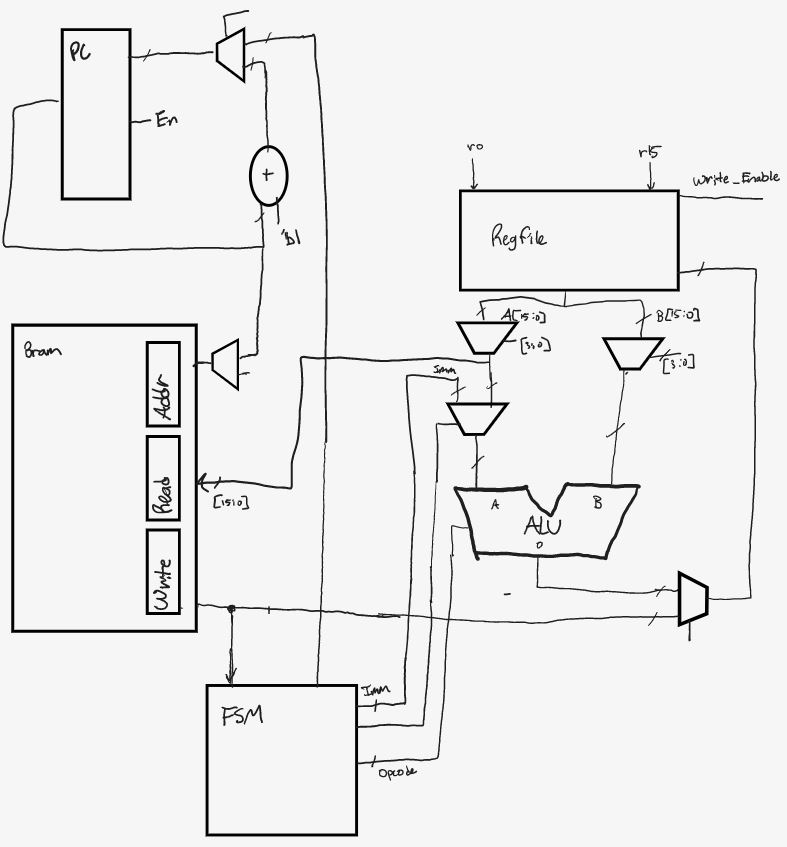
\includegraphics[scale=0.55]{resources/figures/full_bd.jpg}
    \caption{Full block diagram for the cr16 processor.}
    \label{fig:full_bd}
\end{figure}

\section{Testing With Software}
We wrote a series of test programs designed to test each type of instruction incrementally. We broke those programs down as follows:
\begin{enumerate}
    \item \textit{ALU instructions:} We wrote a couple of simple programs to test ALU operations.
    \begin{enumerate}
        \item add\_fibonacci.dat: Uses ADD and ADDI instructions to calculate 5 digits of the Fibonacci series.
        \item mul\_powers2.dat: Uses MUL and MULI instructions to display powers of 2.
        \item logic.dat: Uses a combination of AND, OR, NOT, XOR, ARSH, ALSH, RSH, and LSH instructions to test logic exhaustively.
    \end{enumerate}
    These tests can be viewed in the demo video submitted for the first checkoff.
    \item \textit{Memory interfacing instructions:} We wrote two programs to test MOV, LOAD, and STORE instructions. These programs calculate 4 digits of the Fibonacci series and shuffle them between memory and the regfile.
    
    While testing these instructions we determined that the memory space would use a dedicated stack pointer, defined as r15 in Table 2 of the appendix. The stack will grow from the highest address in BRAM to the lowest. We should have plenty of memory space so as not do overwrite instructions, but since we use 16-bit addresses, we can always expand our BRAM capacity.
    \item \textit{Control flow instructions:} We wrote a bank of 7 tests for each Bcond and Jcond to exhaustively test each condition. Each test performs some meaningless operations with "for" loops, "while" loops, and if-then-else statements. We have found that each of these works properly.
\end{enumerate}
All tests can be found within the "src/asm" directory of our project repository.

\section{Synthesis Reports}
\begin{figure}[t]
    \centering
    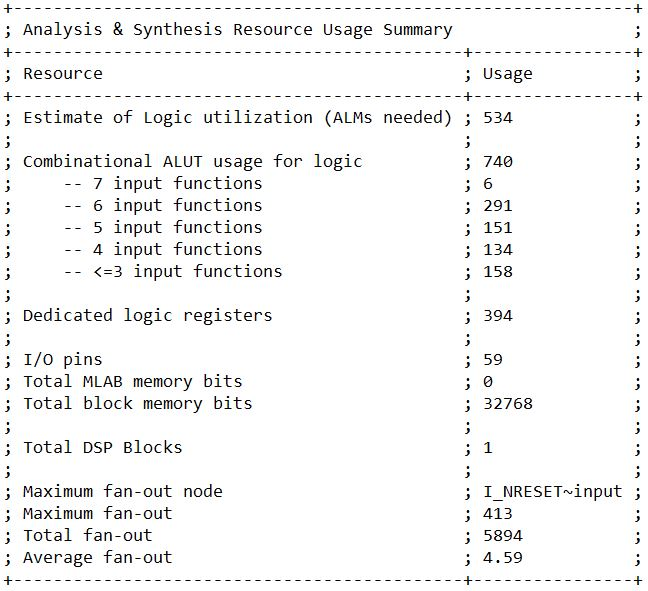
\includegraphics[scale=0.65]{resources/figures/resource_summary.jpg}
    \caption{Resource Summary from the Quartus mapping synthesis report.}
    \label{fig:resource_summary}
\end{figure}

The resource use of the cr16 design is detailed in Fig. \ref{fig:resource_summary}. Of course we don't occupy nearly the maximum ALUT capacity of the FPGA. We can see clearly that our unit uses 32,768 bits (4KB). This will likely be enough memory to accomplish our needs, but we may not know until we have written our code. Since we have established 16-bit addresses, we can expand the memory if needed.

There is a very large amount of fan-out coming from the master reset signal I\_NRESET, which is tied to essentially every register in the hardware. There is potentially a lot of power loss that can be attributed to this, but this signal will inevitably have a lot of fan-out. Despite that large fan-out, the average fan-out of the whole system is 4.59. We are not too concerned with the power usage of this device as our attention shifts to the construction of the FSS hardware.
\section{Timing Analysis}
Meaningful timing analysis is a little challenging with sequential logic, so we have run the the timing analyzer on just the cr16 module. We set it to measure just propagation delay, and the results were as expected. Since the fanout is so high on the I\_NRESET signal, we would expect it to have the longest propagation delays. This can be seen in Fig. \ref{fig:prop_delay}. Hopefully if we run into any clock and timing issues with our FSM and the 50MHz FPGA clock, we can get some debugging help, but our current tests have not exposed any potential timing issues in that regard.

\begin{figure}[t]
    \centering
    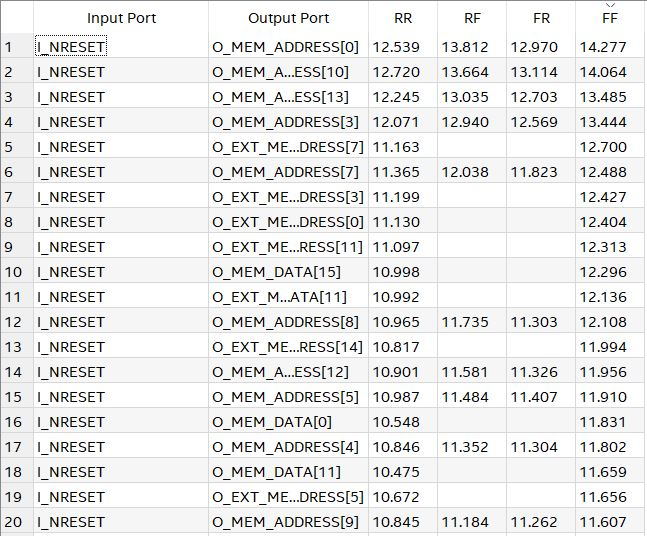
\includegraphics[scale=0.65]{resources/figures/prop_delay_cr16.jpg}
    \caption{Quartus Timing Analyzer output for propagation delay on combinational paths within cr16.}
    \label{fig:prop_delay}
\end{figure}

\section{Note on the Assembler}
Since we heavily modified the provided ISA, we believe it is necessary to write our own assembler. This is not currently complete, so we have no results to report, but we will address briefly some design obstacles that the assembler will have to handle. First, the assembler will have to keep track of line numbers to count displacements properly, so we have to decide how to handle labels in our assembly code. We will also have to decide all the conventions of the assembly language such as how to write registers, whether or not to include commas, and whether or not to lead immediates with a character like a '\$'. These decisions will come this weekend as we put together the finishing touches on the cr16. Some of the software convention decisions such as register naming conventions and jump condition encoding are contained in Appendix Table 2 \& 3.

\section{Conclusion}
Our cr16 processor is nearly completely equipped for our application. Moving forward, we have to finish the implementation of CALL, CALLD, RET, PUSH, and POP instructions. These things will be implemented this weekend, along with support for all instructions in our custom assembler. We will also be setting forward a timeline for constructing our device and implementing our software system by the December 9th deadline. The labor in the future will be divided in the following ways:
\begin{enumerate}
    \item Nate Hansen: Lab 4 report, LUT Sine wave software, audio CODEC, test software for cr16.
    \item Jacob Peterson: cr16 Verilog file, I2C protocol software, assembly compiler, Github setup and directory control, ROMBOM parts purchase and inventory, coordinate semi-professional demonstration video.
    \item Isabella Gilman: SolidWorks drawings, physical design of FSS device, PCB design, device assembly.
    \item Brady Hartog: Parts purchase and inventory, PCB design, materials acquisition, contact consultants.
\end{enumerate}

We are excited to see our cr16 at work with our Fully-Synchronized Synthesizer Interface. 



\clearpage
\setboolean{@twoside}{false}
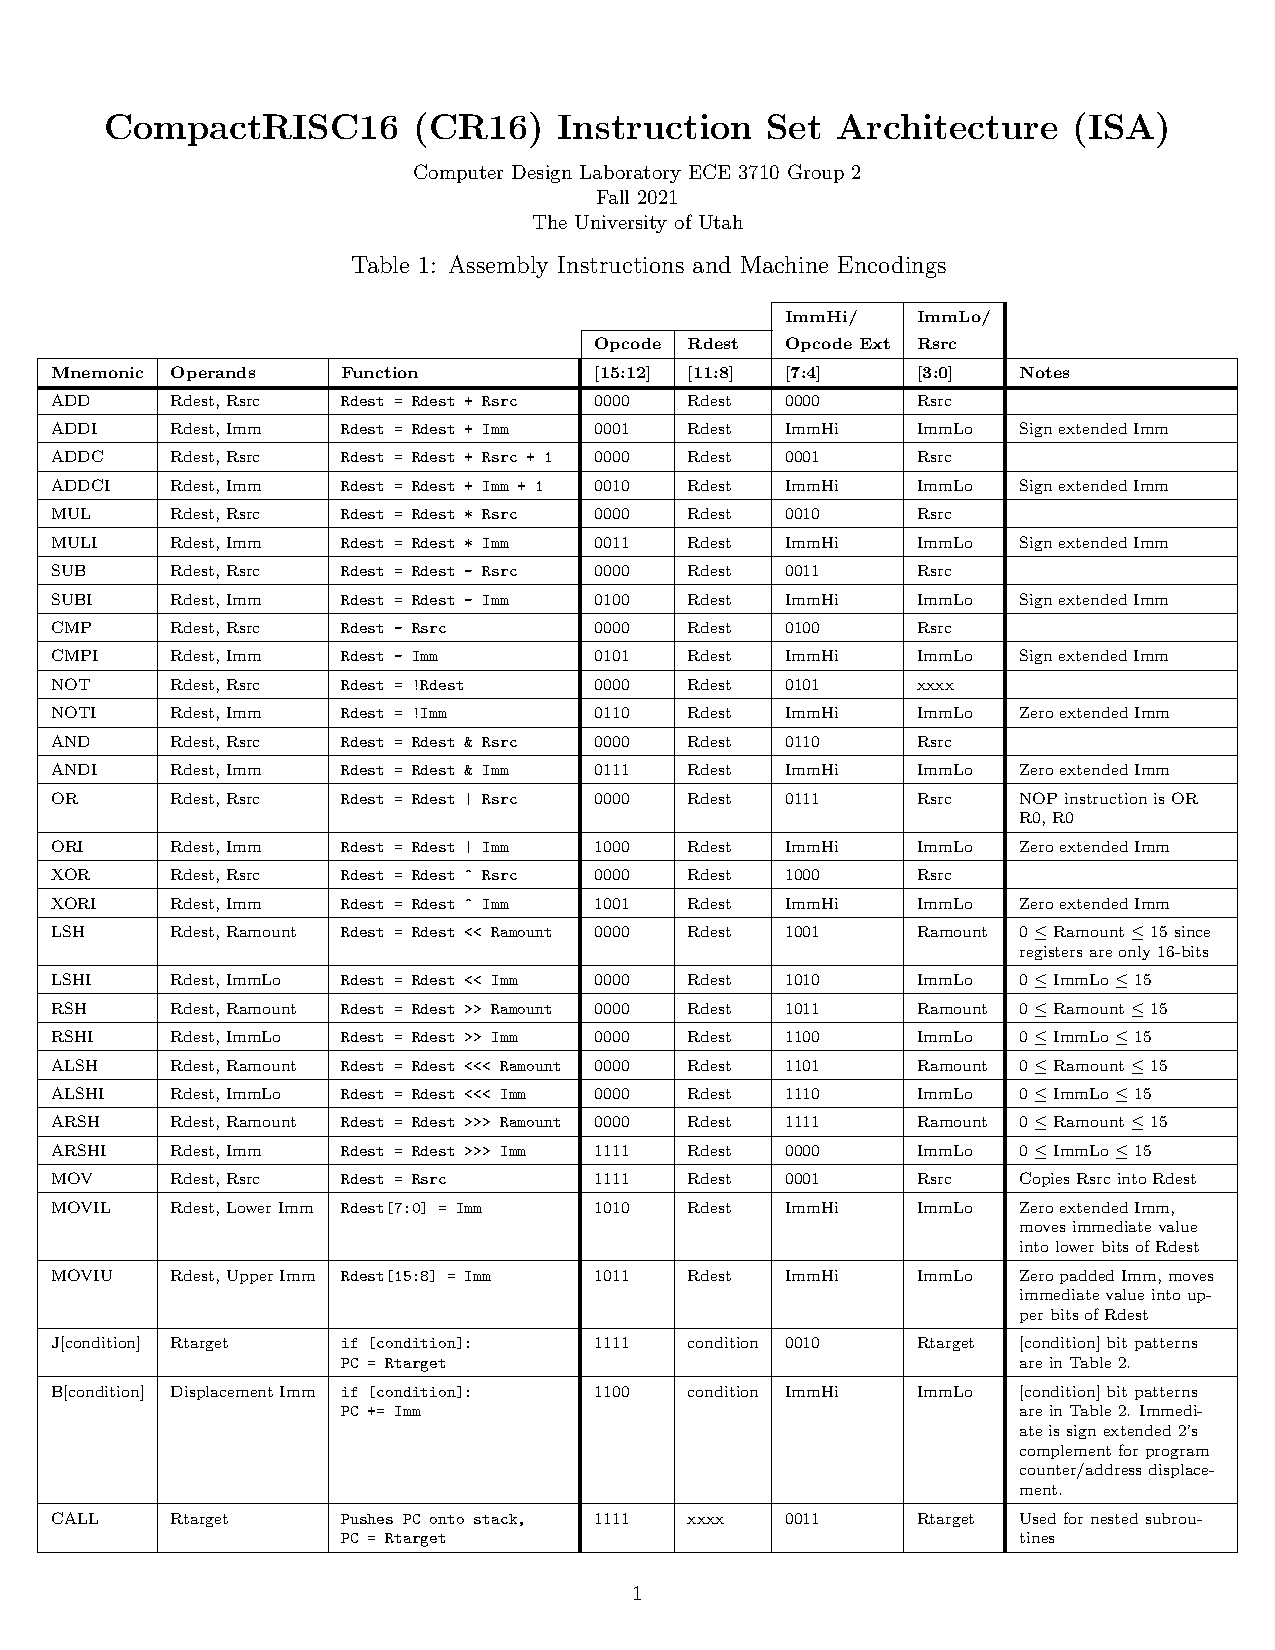
\includepdf[pages=-, offset=0 0]{"../../Datasheets/CR16 ISA/CR16 ISA.pdf"}

\end{document}